\documentclass[10pt,UKenglish]{article}
\usepackage[T1]{fontenc}
\usepackage{lmodern}
\usepackage{fouriernc}
\usepackage[latin9]{inputenc}
\usepackage[a4paper]{geometry}
\geometry{verbose}
\pagestyle{plain}
\usepackage{babel}
\usepackage{graphicx}
\usepackage{amsmath}
\usepackage{setspace}
\onehalfspacing
\usepackage{siunitx}
\usepackage{microtype}
\usepackage{nicefrac}
\usepackage{subfigure}
\usepackage[unicode=true, pdfusetitle, bookmarks=true, bookmarksnumbered=false, bookmarksopen=false, breaklinks=false, pdfborder={0 0 1}, backref=false, colorlinks=false]{hyperref}

\begin{document}

\title{Supplementary theory}
\author{Gen Zhang}
 
\maketitle

\renewcommand{\thesection}{S-\Roman{section}}
\numberwithin{equation}{subsection}

\section{\label{sec:introduction}Background and motivation}

The possibility of proliferative heterogeneity leads us to consider a complicated model of cell fate choice: 
\begin{align}
S &\overset{\Lambda}{\longmapsto} \begin{cases}
S+S & r_S \\
S+A & 1-2r_S \\
A+A & r_S\end{cases} & A &\overset{\lambda}{\longmapsto} \begin{cases}
A+A & r(1-\Delta) \\
A+B & 1-2r \\
B+B & r(1+\Delta)\end{cases} & B &\overset{\gamma}{\longmapsto} \emptyset
\label{eq:really-full-model}
\end{align}
In addition to the parameters above, there are parameters for the proportion of stem cells and \emph{committed progenitors} (CP) in the basal layer, $\rho_S$ and $\rho$ respectively. In addition, whilst we have good evidence <clayton,etc> that CP cells observe a stochastic fate, there is evidence <klein patterning> that stem cells do not and instead have an intrinsically two-dimensional dynamics. However, it is observed that the stem population is long-lived and slow-cycling. This offers the possibility of approximating the stem compartment as also stochastic, which would be statistically exact if stem cell behaviour is uncorrelated on time scales we can observe. In particular, the behaviour should only become correlated if two stem cells are close together; with a low induction rate, this will be negligible. In addition, it is observed <main text> that symmetric division of stem cells is extremely rare, possibly non-existent, in homeostasis.

Thus we are led to consider: 
\begin{align}
S &\overset{\Lambda}{\longmapsto} S+A & A &\overset{\lambda}{\longmapsto} \begin{cases}
A+A & r(1-\Delta) \\
A+B & 1-2r \\
B+B & r(1+\Delta)\end{cases} & B &\overset{\gamma}{\longmapsto} \emptyset
\label{eq:full-model}
\end{align}
In effect, we are looking for statistical evidence of stem cells in CP dynamics --- the latter acts as an amplifier of stem cells. It is then necessary to be as exact as possible about CP dynamics. For this purpose, we focus on the model introduced in <Clayton> of CP cells with balanced fate:
\begin{align}
A &\overset{\lambda}{\longmapsto} \begin{cases}
A+A & r \\
A+B & 1-2r \\
B+B & r\end{cases}, & B &\overset{\gamma}{\longmapsto} \emptyset.
\label{eq:basal-model}
\end{align}
We proceed then to quantify the parameters of this model in section \ref{sec:suprabasal-inference}, before considering the stem compartment as a perturbation in section \ref{sec:stem}. <Harvard> has given a comprehensive study of model \ref{eq:basal-model}. In the limit of large time, i.e. $t\rightarrow \infty$, there is a linear growth of surviving clones $$\left\langle n^\textrm{surv.} \right\rangle = \frac{t}{\tau},$$ where the characteristic time scale $\tau = \rho/r\lambda$, with $\rho = \gamma/(\lambda+\gamma)$ being the equilibrium proportion of CP cells in the basal layer. In addition, the surviving clone size distribution tends to a scaling limit: $$P^\textrm{surv.}_n(t) = \frac{1}{\left\langle n^\textrm{surv.} \right\rangle}\exp\left(-\frac{n}{\left\langle n^\textrm{surv.} \right\rangle}\right).$$ <Harvard> shows that this scaling limit is approached quickly, and becomes very good as soon as $t/\tau$ reaches a few.

The reason for this is that in the large time limit, $\left\langle n^\textrm{surv.} \right\rangle$ becomes large, thus most clones are macroscopic and fluctuations are negligible. In particular, the limiting proportion $\rho$ is attained. Thus, the differentiated basal cells (B) are completely slave to the CP cells' dynamics, and we reduce to the even simpler model <klein>: 
\begin{align}
D &\overset{1/\tau}{\longmapsto} \begin{cases}
D+D & \frac{1}{2} \\
\emptyset & \frac{1}{2}\end{cases}\label{eq:simple-balanced-model}.
\end{align}
This is a classic \emph{critical branching process} <atherya>, which is exactly solvable. The average size is $\left\langle n^\textrm{surv.} \right\rangle = 1+t/\tau$. The clone size distribution is geometric at all times: $P^\textrm{surv.}_n(t) \sim x^n$, thus $x = 1 - \left\langle n^\textrm{surv.} \right\rangle^{-1}$.

Although theoretically very attractive, this long-time scaling behaviour is actually unhelpful in so far as inferring the parameters $(\rho, r, \lambda)$ from experimental data. Since after just a few cell divisions the clone distribution becomes a featureless exponential, it is only possible to measure the characteristic time scale $\tau$ (though this may be determined very accurately, see section \ref{sec:ball-plane}). The cycling rate $\lambda$ may be directly measured from observation of proliferation and the proportion of proliferating progenitor cells $\rho$ may be measured from the expression of the genetic marker Ki67. Finally, $r$ may be obtained by inverting the equation $\tau = \rho/r\lambda$. However, these all introduce additional errors, both systematic and random; worse, these errors are difficult to estimate. In particular, if the genetic marker is unreliable or inefficient, then this would have a very direct effect on the inferred value of $r$.

To do better, it is necessary concentrate on the short-time behaviour and the approach to scaling. In section \ref{sec:suprabasal-inference} below, we show that if clone size distributions \emph{with suprabasal counts} are available, then it is possible to directly infer the triplet $(\rho, r, \lambda)$ from the experimental data. The datasets obtained this way are very rich, with complex structure. To fully incorporate the available information, we use a first-principles Bayesian analysis.

Finally in section \ref{sec:stem}, we show that the scaling behaviour is robust even in the presence of a stem cell population, but that single cell clones provide statistical means to infer the parameters of model \ref{eq:full-model}.

\section{\label{sec:suprabasal-inference}Bayesian analysis of clone fate data}

\subsection{Inferring parameters from observations}

Bayes' theorem gives the \emph{posterior distribution} of the parameters $\theta$ as a result of some observations $O$: $$p(\theta|O) = \frac{p(O|\theta)}{p(O)} p(\theta).$$ The factor of $p(O)$ acts as a \emph{normalisation} to make the left-hand side a proper probability distribution and so is biologically uninteresting. 

The \emph{likelihood} $p(O|\theta)$ depends fundamentally on the predicted clone size distributions $P_{mn}$ (see below, section \ref{sec:p-mn-calculation}). The observations $O$ are an unordered list (but with repetition) of cohorts $O_t = \{(m,n)\}$ with $m$ basal cells and $n$ suprabasal cells seen at a time $t$ after induction. We assume that the induction probability is sufficiently low that the initial conditions are essentially just single cell clones. We can filter out induction of suprabasal cells by conditioning $P_{mn}$ on $m \ge 1$, i.e. \emph{floating clones}. Even so, we have an unknown chance of inducing a terminally differentiated cell in the basal layer; we do not want to make extraneous assumptions about induction rates, and filter out such data by conditioning on clones of size 2 or above, i.e. $m+n \ge 2$. The latter criterion also excludes from consideration extinct clones, which are by definition unobservable. As such, we define the \emph{observable clone distribution} $$P^\textrm{obs.}_{mn} = \frac{P_{mn}}{1 - P_{00} - P_{10} - \sum_j P_{0j}}.$$ Now given that the observation $O_t$ is filtered as above, we can compute the likelihood: $$p(O_t|\theta) = \prod_{(m,n) \in O_t} P^\textrm{obs.}_{mn}(t),$$ where the product is intended to repeat factors according to the multiplicity of the pair $(m,n)$.

The only ingredient remaining is the \emph{prior distribution} $p(\theta)$. To be completely rigorous, we should pick it to be a maximum entropy distribution over the parameter space $\theta$ <jaynes>. In this case that means a uniform distribution in $\rho$ and $r$. The rate $lambda$ has no natural scale, and the maximum entropy distribution over $\lambda$ must be invariant under a change of units. Thus we choose a log-uniform distribution, $p(\theta) \propto 1/\lambda$; this is technically \emph{improper}, as it cannot be normalised, but actually causes no real problems --- we only require the final posterior distribution to be proper.

Multiple time points can be combined by simply multiplying the likelihood functions together, since by the very nature of cohort studies there are no correlations between different observations at different times.

Figure \ref{fig:blob} shows a typical example of the inference. The posterior distribution is well-localised distribution. Below, we will incorporate information from the scaling limit.

\begin{figure}[htb]
	\centering
	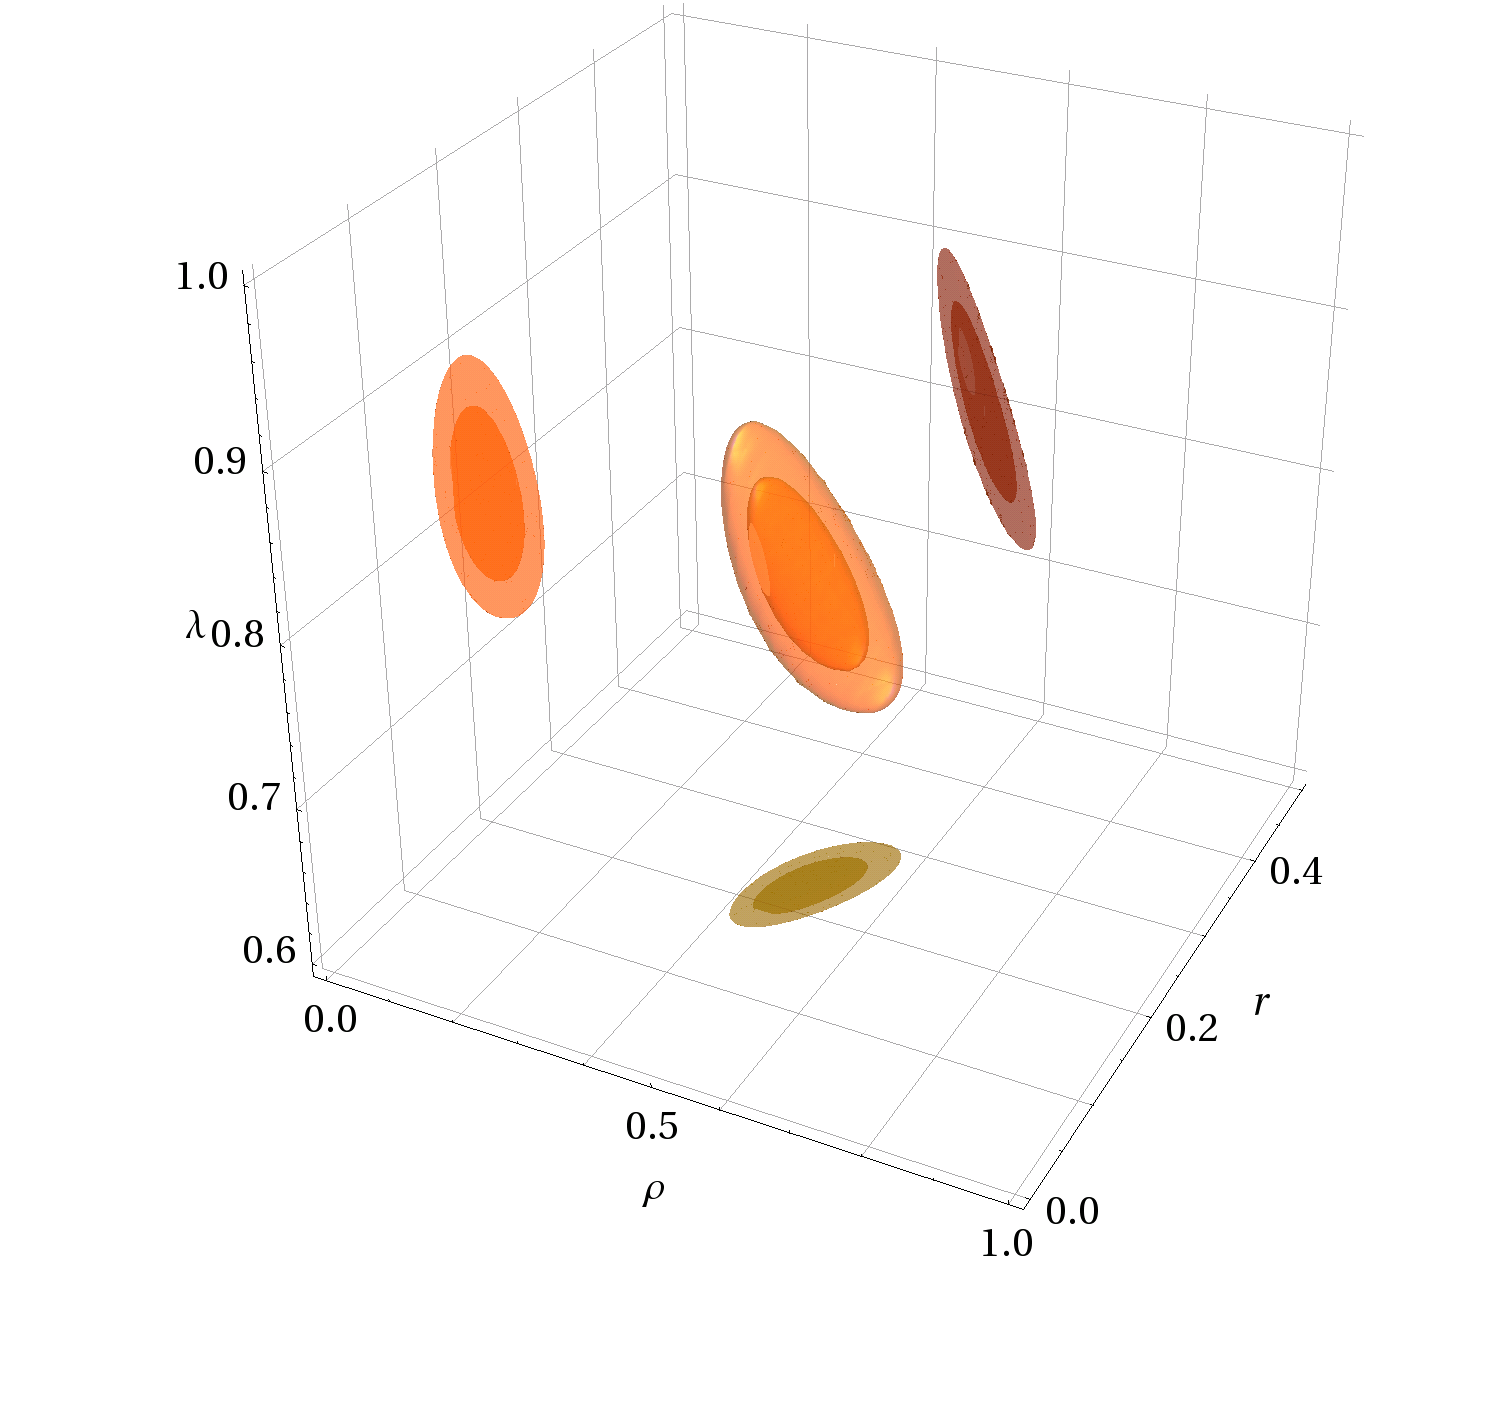
\includegraphics[height=4in]{ABC/oes_eyp_bs_combined_atra_control_cond_prior.png}
	\caption{\label{fig:blob}The posterior distribution upon inference using 22 day and 30 day data with suprabasal counts. Here we plot the $68\%$ and $95\%$ confidence regions, and their projections.}
\end{figure}

\subsection{\label{sec:p-mn-calculation}Clone size distributions with suprabasal cells}

The central prediction of the theory is a distribution $P_{mn}(t)$, the probability of a clone having $m$ basal cells and $n$ suprabasal cells at time $t$ after induction. Since we are tracking suprabasal cells, we will expand the stochastic model \ref{eq:basal-model} to include:
\begin{equation*}
B \overset{\gamma}{\longmapsto} C
\end{equation*}
where suprabasal cells are represented as $C$.

Whilst we cannot experimentally distinguish between proliferating CP cells ($A$) and terminally differentiated cells in the basal layer ($B$), it is necessary to do so mathematically as they produce entirely different progeny trees. Thus we will work with the finer grained distribution $P_{m_A m_B n}$ which is related $$P_{mn} = \sum_{m_A + m_B = m} P_{m_A m_B n}.$$ 

Our model has the Markovian property, which is that the future behaviour only depends on the current state of the system, and not directly on the past history. As with all Markovian systems <cite>, the behaviour can be described by a (infinite) system set of first order differential equations, known as the master equation for the system: 
\begin{equation}
\frac{dP_{m_A m_B n}}{dt} = \sum_{m_A^\prime m_B^\prime n^\prime} T_{m_A m_B n; m_A^\prime m_B^\prime n^\prime} P_{m_A^\prime m_B^\prime n^\prime}. \label{eq:infinite-master}
\end{equation}

Our model also has a special property: the number of cells in a clone can never decrease. This means that $P_{m_A m_B n}(t)$ can only depend on the probabilities of clones with the same or fewer total cells. Thus if we only care about clones up to a certain size we can truncate the infinite set $P_{m_A m_B n}$ to a finite one, and package them up into a vector $\mathbf P$. At the same time, only a finite number of elements of $T$ will be needed, and moving them into a matrix $\mathbf T$ allows the master equation \eqref{eq:infinite-master} to be written compactly as $$\frac{d\mathbf P}{dt} = \mathbf{T P}.$$ This is then a standard differential equation, whose solution is a matrix exponential $$\mathbf P = \exp(\mathbf T t) \mathbf P_0,$$ where $\mathbf P_0$ is the initial condition, i.e. one type $A$ cell.

\subsection{\label{sec:ball-plane}Consistency and improvement with basal statistics}

The need to count suprabasal cells limits the scope of the experiment, as eventually shedding becomes a serious effect, and its statistical effects are likely to be environmentally dominated. Counting basal statistics only, it becomes possible to extend the experiment to longer time scales and accurately measure the scaling behaviour. This would then provide both a consistency check of the methodology and also extra information with which to improve the inference. Whilst it would be straightforward to extract $\tau = \rho/r\lambda$ as shown in <klein>, it is also worthwhile to run a full-scale Bayesian analysis, and combine this with the inference from short-time suprabasal data.

Fundamentally, there is very little change in the procedure already described above. The main difference is that the branching model \ref{eq:basal-model} does not enjoy the triangular structure which allowed the probabilities to be computed simply via a matrix exponential, and the full infinite system must be treated. The basal distributions $P_m$ are best computed via generating function methods, e.g. <tedious paper; maybe there should be a section here to explain how to do it?>. It is also possible to do a simple truncation, but the errors are difficult to bound. Either way, it is possible to calculate the likelihood function $p(O|\theta)$.

As mentioned in the introduction (section \ref{sec:introduction}), the basal statistics quickly converge to the scaling limit. In this limit, all choices of parameters which give the same time scale $\tau=\rho/r\lambda$ would give the same predictions, and thus would be indistinguishable. The posterior distribution (figure \ref{fig:inferences}, main text) is tightly concentrated along the hyperbolic sheet defined by some particular value of $\tau$. There is a small amount of variation within the sheet; it seems that the basal statistics does contain some non-scaling information, mostly within the early time points. This is a good example of the sensitivity of Bayesian analysis.

Consistency between basal and basal-plus-suprabasal statistics manifest as non-trivial overlaps of significant parts of the respective posterior distributions. These estimates may then be combined by the usual multiplication of likelihoods (figure \ref{fig:inferences}, main text).

\subsection{Meaning of posterior probabilities}

It is important to be clear about what the 95\% confidence region in figure \ref{fig:blob} means. The exact statement is that \emph{given the correctness of the underlying model, there is only a 1 in 20 chance that the data collected is perverse to the extent that the true parameters of the model lie outside of the region}.

<inference of MC-generated data; shows spread in inferred ball locations>

Although the posterior distribution is nicely peaked, it would be a mistake to think that the true parameters are more likely to be at the most probable value, as opposed to some definite distance away from the peak. This can be clearly seen in figure \ref{fig:blob} above, where the true parameters are actually never very close to the centres of the confidence regions. This can be understood very simply as a consequence of multi-dimensional distributions. For example, if we had a three-dimensional Gaussian $$p(\mathbf{r}) \propto \exp\left(-|\mathbf r|^2\right),$$ the expectation $\left\langle \mathbf |\mathbf r| \right\rangle > 0$ and is in fact of the order of the standard deviation. In section \ref{sec:ball-plane}, when we look for consistency against long time course basal statistics, we should not be surprised that the hyperbolic sheet does not exactly intersect the centre of the ball.

\section{\label{sec:stem}Impact of stem cell population}

Previously, we have analysed the data on the basis that only CP cells proliferatively contribute. However, the existence of a long-lived, slow-cycling stem population has the potential to change the clone size distribution. Indeed one of the most significant traits is the relative enrichment of single cell clones --- interpreted as a single stem cell which was induced but then never divided <main text>. Here, we show that deviations from the balanced CP model (\ref{eq:basal-model}) are small, and essentially constrained to a very slight increase in small clones, but well within currently achievable statistical errors.

Fundamentally, if stem cells can differentiate to committed progenitors, then the CP dynamics must be slightly imbalanced --- otherwise homoeostasis would be violated. At the same time, for the stem cells to be only slowly cycling, the asymmetry must be very small. Figure <main text> shows that the balanced CP process is an excellent fit to the data, therefore, any deviation must be very small. This would be all consistent with the hypothesis that stem cells are recruited for repair <wounding cite>, but are otherwise quiescent in normal tissue.

This slow turn-over means that we do not expect to be able to statistically resolve the stem cell dynamics; only changes in the CP dynamics will be measurable. In the limit of small numbers of active stem cells, the main effect will be a random injection of a CP cell into an existing clone: 
\begin{equation}
S \overset{\Lambda}{\longmapsto} S+A. \label{eq:stem-division-model}
\end{equation}
This is a mathematical simplification and, to within accessible statistics, is exact in the limit. It does not imply a biological assumption of stochasticity; in particular, we are not ruling out other dynamics of the stem population, which must necessarily include self-renewal and environmentally controlled division to produce the patterning observed (figure <main text>).

Since the imbalance is small, we expect that at short times the dynamics is essentially the same as the balanced case. Thus if we only care about the long time behaviour, i.e. large clones, we can (like in model \ref{eq:simple-balanced-model}) neglect fluctuations of $\rho$ and simplify the CP dynamics to be
\begin{equation}
A \overset{\lambda}{\longmapsto} \begin{cases}
A+A & r(1 - \Delta) \\
A & 1 - 2r \\
\emptyset & r(1 + \Delta)
\end{cases}\label{eq:subcritical-cp-model}
\end{equation} which allows analytical treatment.

We now have three extra parameters to determine: the \emph{active stem cell proportion} $\rho_S$, the mean stem cell division rate $\Lambda$ and the imbalance (and so CP loss rate) $\Delta$. We shall see that these may be determined from the statistical data available, although with uncertainties due to fluctuations in induction efficiency.

Due to the low induction frequency and low proportion of cycling stem cells, we expect each clone contain at most one stem cell. Thus we have two cases to consider: clones with no stem cells at all, which will all eventually go extinct, and clones with one stem cell which will equilibrate at some finite clone size. Below, we take these cases separately.

\subsection{Subcritical CP dynamics}

Model \ref{eq:subcritical-cp-model} is a \emph{subcritical branching process} <cite>. The expected clone size decreases monotonically $\langle n \rangle = n_0 e^{-2 r \Delta \lambda t}$, i.e. we lose cells at a rate of $2 r \Delta \lambda$. Define
\begin{align*}
\beta &= \frac{\left(1-e^{-2 r \Delta \lambda t}\right)(1-\Delta)+2\Delta}{2\Delta}.
\end{align*}
The clone size distribution is:
\begin{equation*}
P_m(t) = \begin{cases}
1 - \frac{e^{-2 r \Delta \lambda t}}{\beta} & m=0 \\
\frac{e^{-2 r \Delta \lambda t}}{\beta} \frac{1}{\beta-1} \left(1-\frac{1}{\beta}\right)^m & m\ge1
\end{cases}
\end{equation*}
Note that the distribution is geometric for $m \ge 1$, and the surviving average clone size $\left\langle n^\textrm{surv.} \right\rangle = \beta$. This information can be packaged up into a single \emph{generating function} $f(z,t) = \sum_m P_m(t) z^m$:
\begin{equation*}
f(z,t) = \frac{e^{2 r \Delta \lambda t}\left[(1-z) + (1+z)\Delta\right] + (z-1)(1+\Delta)}{e^{2 r \Delta \lambda t}\left[(1-z) + (1+z)\Delta\right] + (z-1)(1-\Delta)}.
\end{equation*}

\subsection{\label{sec:subcritical-immigration}Stem supported clones}

Homoeostasis requires that the loss of CP cells be balanced by creation via stem cell division. If the overall cycling stem population as a proportion of all basal cells is $\rho_S$, then we must have $$\rho_S \Lambda = (1-\rho_S) \times 2 r \Delta \lambda.$$ The division process \ref{eq:stem-division-model} preserves the number of stem cells and each of the created CP cells go on to divide and differentiate independently.

Consider then a stem cell which undergoes asymmetric division $n$ times within a time $t$, at times $t_1 < t_2 < \ldots < t_n$. Since the process is Poisson, the probability of having $n$ divisions is independent of when they occur, and is $\Lambda^n e^{-\Lambda t}$. The generating function for the distribution of CP cells for such a sequence of divisions is then
\begin{align*}
g_n(z,t) &= \Lambda^n e^{-\Lambda t} \int_0^t dt_1 \int_{t_1}^t dt_2 \ldots \int_{t_{n-1}}^t dt_n f(z,t-t_1) \times f(z,t-t_2) \times \ldots \times f(z,t-t_n) \\
 &= \frac{\Lambda^n e^{-\Lambda t}}{n!} \left[\int_0^t f(z,t-\tau) d\tau \right]^n
\end{align*}
where we notice that the need to order the times $t_n$ can be removed since it just results in an over counting. The generating function for the number of CP cells in total is then
\begin{align*}
g(z,t) &= \sum_n g_n(z,t) \\
 &= e^{-\Lambda t} \exp\left[\Lambda \int_0^t f(z,t-\tau) d\tau \right] \\
 &= \exp\left\{\Lambda \int_0^t \left[f(z,\tau) - 1\right] d\tau \right\} \\
 &= \exp\left(\frac{4 r \Delta \Lambda t}{1-\Delta}\right) \left\{ \frac{\left(e^{2 r \Delta \lambda t}-1 \right)(z-1)}{2\Delta} + \frac{1}{2}\left[(1-z) + e^{2 r \Delta \lambda t}(1+z) \right]\right\}^{-2\Delta\Lambda/\lambda}.
\end{align*}

The distribution $P_m$ may be obtained by computing the coefficients of the Taylor expansion $$g(z,t) = \sum_m P_m(t) z^m.$$ In this case, exact expressions are not easily available, but are still numerically efficient to extract. Note that since the function $g(z,t)$ has a branch point in the $z$ complex plane, the radius of convergence of the Taylor expansion has a finite radius of convergence $R$. In addition, $$g(z=1,t) = \sum_m P_m(t) = 1,$$ the radius of converge $R \ge 1$. The ratio test for convergence gives $$\lim_{m\rightarrow \infty} \left| \frac{P_{m+1}}{P_m} \right| = \frac{1}{R},$$ thus for large $m$, the distribution becomes geometric.

\subsection{Mean clone size}

As mentioned, the imbalance $\Delta$ is very small, and we expect that short time dynamics is essentially the same as the balanced case. Further, we expect that major deviations only occur on time scales $1/\Lambda \sim 1/2 r \Delta \lambda$.

Experimentally, we induce single cells. These may be either a CP or a stem cell. Assuming proportional induction, the generating function for the total distribution is $$h(z,t) = \rho_S z g(z,t) + (1-\rho_S) f(z,t).$$ The factor of $z$ simply accounts for the fact that each stem-derived clone will contain one stem cell. The average clone size, by construction, is constant. The observed average size will still increase, since extinct clones will not contribute: 
\begin{align*}
\left\langle n^\textrm{obs} \right\rangle &= \frac{1}{1 - h(z=0)} \\
  &= \frac{1}{\rho_S + \beta (1-\rho_S) e^{-2 r \Delta \lambda t}}.
\end{align*}
At early times, we have the linear growth characteristic of a critical branching process, before reaching a plateau at $1/\rho_S$ as $t\rightarrow\infty$. The turn over occurs, as expected, around $1/\Lambda$. Since the long time basal data, out to a year, does not show any sign of a plateau, we can infer an upper bound for imbalance $\Delta$.

<figure showing difference>

\subsection{Basal distribution}

Given the generating function <ref>, we can numerically extract the clone size distribution. As we shall see, the existence of a stem cell compartment is still consistent with the experimental observations.

Heuristically, we can understand why there is almost no change. As mentioned in section \ref{sec:subcritical-immigration}, the distribution for stem-supported clones has a exponential tail. This remains true for the equilibrium distribution. Upon scaling, this tail dominates the observable clones; deviations from this exponential distribution is only visible in small clones. Furthermore, this exponential tail is weaker than the tail from the near critical CP sector, and so is drowned out.

<figure show that the stem compartment makes no difference to the clone size distributions; maybe a figure to show the final equilibrium distributions?>

\section{Main text}

<paragraphs in the main text go here>

\begin{figure}[htb]
	\centering
	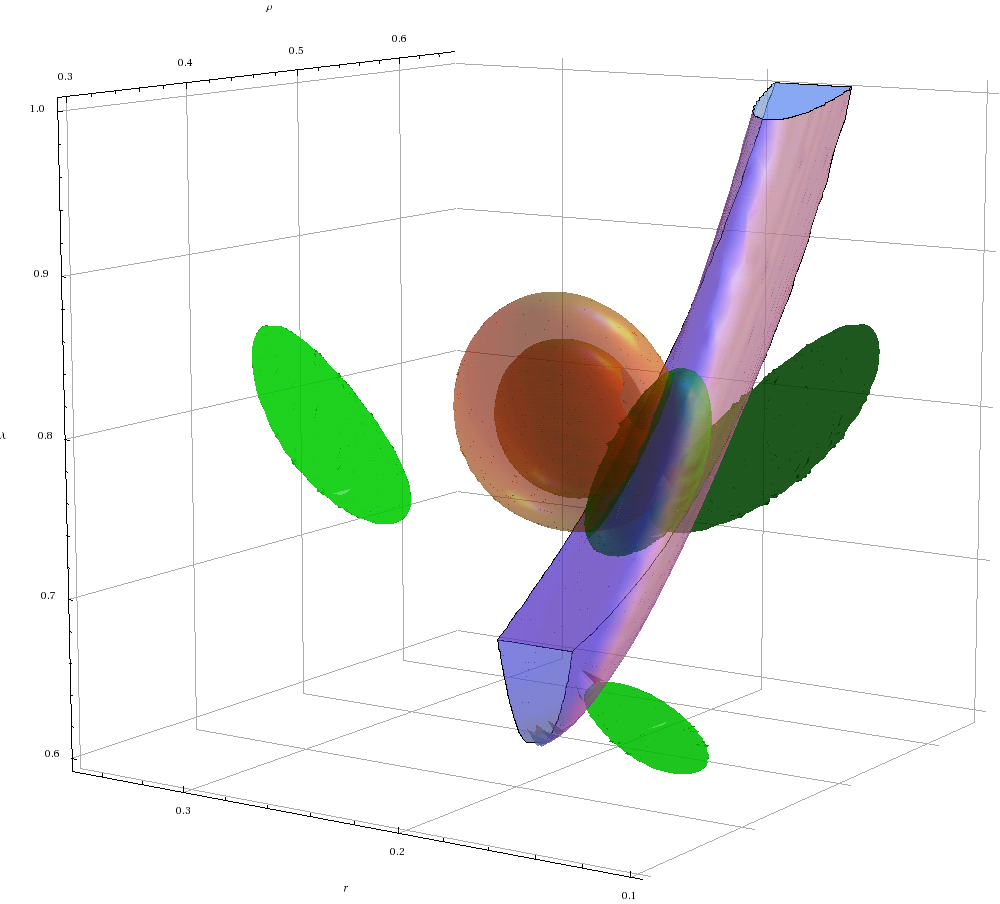
\includegraphics[height=4in]{oes-combined-prior.png}
	\caption{\label{fig:inferences}The inference from short time suprabasal data is in orange, showing $68\%$ and $95\%$ confidence regions. The inference from long time basal data is show in blue. The combined data produces the region ($95\%$) shown in green, with projections shown on the axes planes.}
\end{figure}

\subsection{Single cell clones}

\end{document}
